% This must be in the first 5 lines to tell arXiv to use pdfLaTeX, which is strongly recommended.
\pdfoutput=1
% In particular, the hyperref package requires pdfLaTeX in order to break URLs across lines.

\documentclass[11pt]{article}

% Remove the "review" option to generate the final version.
\usepackage[review]{acl}

% Standard package includes
\usepackage{times}
\usepackage{latexsym}

% For proper rendering and hyphenation of words containing Latin characters (including in bib files)
\usepackage[T1]{fontenc}
% For Vietnamese characters
% \usepackage[T5]{fontenc}
% See https://www.latex-project.org/help/documentation/encguide.pdf for other character sets

% This assumes your files are encoded as UTF8
\usepackage[utf8]{inputenc}

% This is not strictly necessary, and may be commented out,
% but it will improve the layout of the manuscript,
% and will typically save some space.
\usepackage{microtype}

% If the title and author information does not fit in the area allocated, uncomment the following
%
%\setlength\titlebox{<dim>}
%
% and set <dim> to something 5cm or larger.

%algo packages
\usepackage{algorithm}
\usepackage{algorithmic}

%color packages
\usepackage{xcolor}
\colorlet{shadecolor}{orange!15}
\usepackage{color,soul}
\usepackage{soulutf8}
\definecolor{bordeau}{rgb}{0.3515625,0,0.234375}

% position of figure
\usepackage[absolute,overlay]{textpos}

%graphic packages
\usepackage{graphicx}
\graphicspath{ {figures/} }
\usepackage{wrapfig}
\usepackage{float} 
\usepackage{tikz}
\usepackage{pgfplots}
\usepackage{pgfplotstable}

% table packages
\usepackage{array}
\usepackage{multirow,booktabs}
\usepackage{multicol}
\usepackage{tabularx}

% font package
\usepackage[utf8]{inputenc}	% Para caracteres en español
\usepackage{textcomp}
%\usepackage{times}
%\usepackage{lmodern}
\usepackage{mathptmx}

% equation packages
\usepackage{amsmath,amsthm,amsfonts,amssymb,amscd}
\usepackage{mathrsfs}

\usepackage{enumitem}
\setlist{nosep}
\usepackage{latexsym}
\usepackage{graphicx}
\usepackage{xcolor}
\usepackage{longtable}
\usepackage{tikz}
\usetikzlibrary{calc}
\usepackage[draft]{todo}
\usepackage[normalem]{ulem}
\usepackage{xspace}
\usepackage{amsmath,amsfonts,amssymb}

\newcommand{\fyTodo}[1]{\Todo[FY:]{\textcolor{orange}{#1}}}
\newcommand{\fyTodostar}[1]{\Todo*[FY:]{\textcolor{orange}{#1}}}
\newcommand{\fyDone}[1]{\done[FY]\Todo[FY:]{\textcolor{orange}{#1}}}
\newcommand{\fyFuture}[1]{\done[FY]\Todo[FY:]{\textcolor{red}{#1}}}
\newcommand{\fyDonestar}[1]{\done[FY]\Todo[FY:]{\textcolor{orange}{#1}}}
\newcommand{\jcTodo}[1]{\Todo[JC:]{\textcolor{red}{#1}}}
\newcommand{\jcDone}[1]{\done[JC]\Todo[JC:]{\textcolor{red}{#1}}}
\newcommand{\revision}[1]{\textcolor{black}{#1}}
\newcommand{\revisiondone}[1]{\textcolor{black}{#1}}
\newcommand{\revisiondel}[1]{}
\newcommand{\src}{\ensuremath{\mathbf{f}}} % source sentence
\newcommand{\trg}{\ensuremath{\mathbf{e}}} % target sentence
\newcommand{\domain}[1]{\texttt{\textsc{#1}}}
\newcommand{\system}[1]{\texttt{{#1}}}
\newcommand{\SB}[1]{\textbf{#1}}
\newcommand{\SW}[1]{\underline{#1}}
\newcommand{\mtsquare}[0]{MT$^2$}

\title{Multi-domain, multilingual translation with latent multi-task group dropout}
\title{Latent group dropout for multilingual and multidomain machine translation}
% Author information can be set in various styles:
% For several authors from the same institution:
% \author{Author 1 \and ... \and Author n \\
%         Address line \\ ... \\ Address line}
% if the names do not fit well on one line use
%         Author 1 \\ {\bf Author 2} \\ ... \\ {\bf Author n} \\
% For authors from different institutions:
% \author{Author 1 \\ Address line \\  ... \\ Address line
%         \And  ... \And
%         Author n \\ Address line \\ ... \\ Address line}
% To start a seperate ``row'' of authors use \AND, as in
% \author{Author 1 \\ Address line \\  ... \\ Address line
%         \AND
%         Author 2 \\ Address line \\ ... \\ Address line \And
%         Author 3 \\ Address line \\ ... \\ Address line}

\author{First Author \\
  Affiliation / Address line 1 \\
  Affiliation / Address line 2 \\
  Affiliation / Address line 3 \\
  \texttt{email@domain} \\\And
  Second Author \\
  Affiliation / Address line 1 \\
  Affiliation / Address line 2 \\
  Affiliation / Address line 3 \\
  \texttt{email@domain} \\}

\begin{document}
\setlength{\abovedisplayskip}{3pt}
\setlength{\belowdisplayskip}{3pt}
\maketitle

\begin{abstract}
  [FY] Multidomain and multilingual machine translation often rely on parameter sharing strategies, where large portions of the network are meant to capture the commonalties of the task at hand, while smaller parts are reserved to model the peculariaties of a language or a domain. In adapter-based approaches, these strategies are hard coded in the network architecture. In this work, we propose a new method aimed at learning the parameter sharing pattern, using a latent-variable model. We show how this model can be trained end to end, and report experimental results which show that the learned pattern are both meaningful, and yield improved translation performance without any increase of the model size. 
\end{abstract}

\section{Introduction}
Multidomain and multilingual machine translation aim to develop one single model to perform translations for multiple domains and multiple language pairs, respectively.\footnote{We will refer to these two situations as 'multi-task MT' (or \mtsquare{} for short), and refer to individual domains and languages as 'tasks'.} These paradigms are motivated by the compactness of the resulting translation system \citep{dabre20survey,Chu18multilingual}, the hypothetical positive knowledge transfer between similar domains \citep{Pham21revisiting} or between languages in the same family \citep{Tan19multilingual}. However, having all the tasks use exactly the same model parameters can cause negative interference between unrelated tasks \citep{conneau20unsupervised,wang20negative}. Hence the recent development of approaches relying on a partial sharing of the parameters, eg.\ using adapter layers as studied in \citet{houlsby19parameter,Bapna19simple,Pham20Study}. If these techniques have proven effective to achieve strong baselines, such fail to fully take advantage of the similarities that exist between domains and tasks, as documented eg.\ in \citep{Pham21revisiting}. This is because the partition of the parameter space between generic or task-specific sub-parts, and their allocation to each task is hard coded in the network, irrespective of the existing commonalties and differences in the data space.   

In this paper, we try to develop techniques that can take the similarity between tasks into account in a more effective way, by learning the network organization from the data. To this end, we introduce a set of latent variables in the model, to account for the unseen association between tasks and regions of the parameter space, and show how training can still be performed end-to-end using a variational surrogate of the standard loss function. Our experiments with multilingual and multidomain confirm that this method can automatically detect similarities in the data, and yield related tasks to share more parameters. They also show that this method is comparable to using adapter layers in a number of empirical comparisons; contrarily to adapters, these performance are obtained without any increase of the model size.  Our main contribution are summarized below:
\begin{itemize}
  \setlength{\itemsep}{1pt}
  \setlength{\parskip}{0pt}
  \setlength{\parsep}{0pt}
\item We provide a rigorous mathematical formulattion to the problem of jointly learning routing task-dependent sub-networks and the parameters of the underlying models using variational probabilistic modeling;
\item We introduce algorithms to train this model end to end with very little extra computational cost.
\item We report, using an extensive experimental setting, significant gains of this method with respect to strong baselines.
\item We study how this method can actually exploit the similarities between tasks to learn consistent sub-networks.
\end{itemize}

\fyTodo{Can you do distillation ? That is only keep the parameter for one domain and still get good results (better than DA ?)}

\section{Multi-task group dropout \label{sec:architecture}}
\subsection{Network architecture, groups and layers}
Most architectures for multitask learning are based on a matching of subset of model parameters with tasks. While our model also needs to know the task $d \in [0 \dots n_d-1]$ for each training and test instance, the structure of our Transformer networks \citep{Vaswani17attention} is emphbased on the notion of \emph{groups of parameters}. In each Transformer layer $l \in [1 \dots L]$, we identify $n_p$ groups of parameters.\fyTodo{In the attention heads only? In the FF?} The assignment of tasks to groups will be learned from the data, under the constraint that each task has only access to exactly $k$ groups of \emph{active parameters}, while the all the other parameter values are deemed to be \emph{dropped} (see Figure~\ref{fig:group_dropout}).
\begin{figure}
  \centering
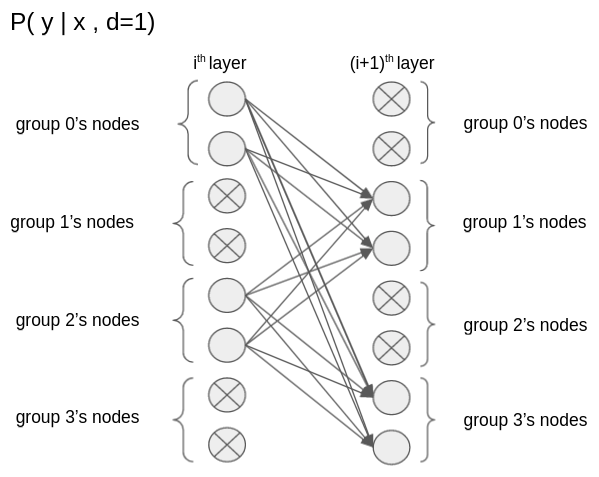
\includegraphics[width=0.4\textwidth]{group_dropout}
\caption{Latent group dropout. The set of nodes\fyTodo{parameters ?} in each layer is divided into equal-sized groups. For a task, we only keep a fixed number of groups. Our method learns which groups will be kept / dropped for each task.}
\label{fig:group_dropout}
\end{figure}
Formally, we define the \emph{group dropout mask} $m_d^l$ as a $n_p$-dimensional binary vector containing exactly $k$ ones: the group $p$ ($\in  [0,\dots,n_p\text{-}1]$) is retained for task $d$ if $m_l^d(p)\text{\small =}1$ and is dropped if $m_l^d(p)\text{\small =} 0$. We denote $\Delta^{n_p}_k = \{ m \in \{0,1\}^{n_p} \text{such that}  \mid{} m \mid_{L_1} = k \}$, where $\mid{} m \mid_{L_1}$ is the $L_1$ norm, the set of all admissible dropout masks.

Given $m_l^d$, the parameter mask $r_l^d$ for task $d$ in layer $l$ is then derived as follows:
\begin{align*}
  r_l^d(i) &= \begin{cases}
    1, & \text{if}\ p \times \frac{d_k}{n_p} \leqslant i < (p+1) \times \frac{d_k}{n_p} \\
    & \text{AND} \  m_l^d(p) \text{\small =} 1 \\
    0, & \text{otherwise},
  \end{cases} 
  % p & \in  \{0,\dots,n_p\text{-}1 \}, \\
  % d & \in  \{0,\dots,n_d\text{-}1 \}, \\
  % i & \in  \{0,\dots,d_k\text{-}1 \}, \\
  % m_l^d & \in  \{0,1\}^{n_p} \ \forall d,l \, \\
  % \mid m_l^d \mid_{L_1} & =  k , \\
  % \Delta^{n_p}_k & =  \{ m \in \{0,1\}^{n_p} | \mid m \mid_{L_1} = k \},
\end{align*}
where $d_k$ is the dimension of the hidden state.\fyTodo{Check this} The propagation of information within the network then depends on the current task value and can be formalized as:
\begin{align*}
  r_l^d &\in \{ 0,1 \}^{d_k}, \\
  \tilde{h}^l &= h^l \odot r_l^d ,\\
  h^{l+1} &= \text{LAYER}^{l+1}(h^l) ,\\
  l & \in [0,\cdots, L-1] ,
\end{align*}
where $\text{LAYER}^l()$ represents all the computations in Transformer layer $l$.
% The dropping mask $r_l^d$ is computed as follows
% where $n_p$ is the number of dropout groups; $n_d$ is the number of domains; $d_k$ is the size of Transformer layers; $k$ is the number of retained groups at each layer; $m_l^d$ is a binary vector indicating which group of the nodes of the $l^{th}$ layer is dropped in the sub-network modeling domain $d$. 

\subsection{Training with latent dropout masks}
We incorporate the latent variables $m_{l}^d, l \in[0,\dots,L]$ into the log-likelihood as follows. For the sake of brevity, we denote $m_l^d$ the set of latent variables, \fyTodo{what do you mean here - this is all there is?} and use $x$, $y$, and $\theta$ to refer to the input, output, and parameter vectors, respectively; finally $\Phi^d_i \in \mathbb{R}^{n_p}$ denotes the set of variational parameters in the model:\fyTodo{Again this is too complicated. How about the notations ? Why no $y$ ?}
Use $\phi$ for all the variational parameters.
\begin{align}
\hspace{-3.em}
\text{log} P(y|x,d;\theta) = &\text{log} P(y, m_l^d |x,d;\theta) \text{-} \text{log} P(m_l^d|y, x, d ;\theta) \nonumber \\
= & \displaystyle{\mathop{\mathbb{E}}_{P(m_l^d | \Phi_l^d)}} \big[ \text{log} P(y, m_l^d | x,d;\theta) \text{-} \text{log} P(m_l^d | \Phi_l^d) \big] \nonumber \\
& \quad + KL(P(m_l^d | \Phi_l^d) \parallel P(m_l^d|y, x,\theta,d)) \nonumber \\
\geqslant & \displaystyle{\mathop{\mathbb{E}}_{P(m_l^d | \Phi_l^d)}} \big[ \text{log} P(y, m_l^d | x,\theta,d) \text{-} \text{log} P(m_l^d | \Phi_l^d) \big] \nonumber \\
 = & \displaystyle{\mathop{\mathbb{E}}_{P(m_l^d | \Phi_l^d)}} \big[ \text{log} P(y | x,\theta,m_l^d, d) \big] \label{eq:lower-bound} \\
& \quad - KL \big( P(m_l^d | \Phi_l^d) \parallel P(m_l^d | x,\theta,d) \big) \nonumber \\
 = & \mathcal{L}_{\text{ELBO}}(\theta, \Phi_l^d, x , y). \nonumber
\end{align}
$\mathcal{L}_{\text{ELBO}}(\theta, \Phi_l^d, x , y)$ is a lowerbound of the log-likelihood, known as the evidence lower bound (ELBO) in variational statistics \citep{Diederick14auto}, of our log-likelihood. Our training loss will be $-\mathcal{L}_{\text{ELBO}}(\theta,\Phi_l^d,x,y)$.

The variational distribution of $m_l^d$, $P(m_l^d|\Phi_l^d)$, is defined as follows:
\begin{align}
\hspace{-2.em}
% &\Phi_d \in \mathbb{R}^{n_p} , \nonumber \\
  Ind^d =& \{ i_1, \cdots, i_k \} \sim \text{SRS}(\operatorname{softmax}(\Phi_l^d),k) , \nonumber \\
  m_l^d(i) =& \mathbb{I}(i \in Ind^d) ,\nonumber
\end{align}
with $\text{SRS}(\pi,k)$ denoting the process of sampling $k$ times without replacement from the distribution $\pi$, and $\mathbb{I}$ the indicator function. This choice for the modeling of the latent vector $m_l^d$ is motivated by the Gumbel Top-K trick of \citet{Kool19stochastic}. In addition, we assume that the prior distribution of $m_l^d$ is uniform over the admissible set $\Delta^{n_p}_k$, $P(m_l^d | x, \theta, d) \ \text{=} \ \operatorname{Unif}(\Delta^{n_p}_k)$.

Given these assumptions for the prior distribution and our choice for the variational distribution, the two terms in Eq.~\eqref{eq:lower-bound} can be reformulated as:

\begin{align}
\hspace{-2.em}
T_1 &= \displaystyle{\mathop{\mathbb{E}}_{P(m_l^d | \Phi_l^d)}} \big[ \text{log} P(y | x,\theta,m_l^d, d)  \big] \nonumber \\
&= \displaystyle{\mathop{\mathbb{E}}_{g_l^d(p) \displaystyle{\mathop{\sim}^{\text{i.i.d}}} Gumbel(0,1) \ }} \big[ \text{log} P(y | x,\theta,\tilde{m}_l^d,d) \big] \nonumber
\end{align}
where
\begin{align}
\hspace{-2.em}
g_l^d & \in \mathbb{R}^{n_p} \nonumber \\
g_l^d(p) & \displaystyle{\mathop{\sim}^{\text{i.i.d}}} Gumbel(0,1) \nonumber \\
& \forall p \in \{ 0,\cdots,n_p\text{-}1 \} \nonumber \\
i_1, \cdots, i_k &= Top\_k \ \{ \ g_l^d(0) + \Phi_l^d(0), \cdots, \label{eq:top-k} \\ 
&g_l^d(n_p\text{-}1) + \Phi_l^d(n_p\text{-}1) \ \} \nonumber \\
\tilde{m}_l^d(p) &= \mathbb{I}(p \in Ind^d). \nonumber 
\end{align}
and
\begin{align}
\hspace{-2.em}
T_2 &= - KL \big( P(m_l^d | \Phi_l^d) \parallel P(m_l^d | x,\theta,d) \big) \nonumber \\ 
	&= \mathbb{H} \big[ P(m_l^d | \Phi_l^d) \big] - \text{log}(\#\Delta^{n_p}_k) \nonumber \\ 
	&= \mathbb{H} \big[ P(i_1,\cdots,i_k | \Phi_l^d) \big] - \text{log}(\#\Delta^{n_p}_k) \nonumber \\
	&\geqslant \mathbb{H} \big[ P(i_1 | \Phi_l^d) \big] - \text{log}(\#\Delta^{n_p}_k) \label{eq:entropy}
\end{align}

we prove inequality~\eqref{eq:entropy} in Appendix~\ref{appendix:b}.

Now we go back to our loss function, which is the negative of the lower-bound \eqref{eq:lower-bound}, consisting of 2 terms $-T_1$ and $-T_2$. The inequality \eqref{eq:entropy} shows that an upperbound of $-T_2$ is $\text{log}(\#\Delta^{n_p}_k) - \mathbb{H}(\text{softmax}(\Phi_l^d))$. During training, we maximize the entropy $\mathbb{H}(\text{softmax}(\Phi_l^d))$ as a regularization over the parameters $\Phi_l^d$ of the variational distribution.

Thanks to the Gumbel Top-K trick, we can move the parameters $\Phi_l^d$ into log-likelihood function and get rid of policy gradients, which have been reported to be very unstable \citep{Diederick14auto}. However, the operator Top-K, which defines $\tilde{m}_l^d$ in Equation \eqref{eq:top-k}, is not differentiable. Therefore, we approximate this function by the Soft-Top-K function defined as follows

\begin{align}
\hat{m}_l^d(\tau) &= \displaystyle{\mathop{argmin}_{\substack{
       0 \leqslant m_i \leqslant 1 \ \forall 0 \leqslant i \leqslant n_d\text{-}1 \label{eq:soft-top-k}\\
        1^{T}.m = k
      }}} -(g_l^d+\Phi_l^d)^{T} . m - \tau H_b(m) \\
& \text{in which} \nonumber \\
H_b(m) &= - \sum_i m_i \text{log}(m_i) + (1-m_i)\text{log}(1-m_i) \nonumber 
\end{align}

In Appendix \ref{appendix:a}, we prove that $\lim_{\tau \rightarrow 0}\hat{m}_l^d(\tau) = \tilde{m}_l^d$. Furthermore, we also provide the computation of $\hat{m}_l^d(\tau)$ and prove that $\hat{m}_l^d(\tau)$ is a differentiable function w.r.t $\Phi_l^d$ and that its differentiation can be computed using the implicit differentiation theorem. During training, we approximate $\tilde{m}_l^d$ by $\hat{m}_l^d(\tau)$ by gradually decaying the hyperparameter $\tau$ to $0$. The gradient of the term $T_1$ w.r.t $\Phi_l^d$ is computed via the chain rule as follows:
\begin{equation}
\frac{\partial T_1}{\Phi_l^d} = \frac{\partial T_1}{\hat{m}_l^d(\tau)} \times \frac{\hat{m}_l^d(\tau)}{\Phi_l^d}
\end{equation}
The gradient $\frac{\partial T_1}{\hat{m}_l^d(\tau)}$ is computed via autograd algorithm while $\frac{\hat{m}_l^d(\tau)}{\Phi_l^d}$ is computed via implicit differentiation, as explained in Appendix~\ref{appendix:a}.

We jointly train the Transformer parameters $\theta$ and the parameters of the latent dropping masks $\Phi_l^d$ using the following multi-task loss.\fyTodo{This is repeated}
\begin{align}
\hspace{-0.em}
\mathcal{L}(\theta,\Phi_l^1,\cdots,\Phi_l^k) = \displaystyle{\mathop{\sum}_{d=1}^{k}} \displaystyle{\mathop{\mathbb{E}}_{x \sim \mathcal{D}_s^d,y \sim g^d(x)}} \big[-\mathcal{L}_{\text{ELBO}}(\theta,\Phi_l^d,x,y)\big]
\end{align}

in which $\mathcal{D}_s^d$ is distribution of the task $d$ over the input space $\Omega^d_s$; $g^d: \Omega^d_s \rightarrow \Omega^d_t$ is the mapping function, which our multi-task modern needs to learn, of the task $d$; $-\mathcal{L}_{\text{ELBO}}(\theta,\Phi_l^d,x,y)$ is the ELBO loss, defined in Equation~\ref{eq:lower-bound}.

Finally, during inference, we define the dropping mask for $l^{th}$ layer and task $d$ as follows:
\begin{align*}
  Ind_l^d &= Top_k(\Phi_l^d) \\
  m_l^d &= \mathbb{I}(i\in Ind_l^d),\\
\end{align*}
meaning that we simply pick the $k$ most likely parameter groups for the task at hand, and define the dropout mask accordingly.

\section{Experimental settings}
\subsection{Baselines}
\subsubsection{Multi-domain, multilingual translation}
In both cases, we examine the performance of three following MT systems.
\begin{itemize}
	\item Transformer
	\item Adapter based Transformer
	\item Transformer with multi-task group dropout
\end{itemize}
For the sake of brevity, we put the detailed descriptions of these systems in Appendix \ref{appendix:c}.
\subsection{Datasets}
\subsubsection{Multi-domain translation}
We reuse the same data as the recent work of \citet{Pham21revisiting} in multi-domain translation. For the sake of brevity, we leave most of the details of data in Appendix \ref{appendix:c}.
\subsubsection{Multilingual translation}
We evaluate our model on both one-to-many (O2M) and many-to-one (M2O)
translation tasks. We evaluate models on widely used multilingual translation datasets.
\begin{itemize}
	\item TED8-Related. Following the setting of \citet{Wang20balancing}, we use a subset of translations of \citet{qi18when} between English and eight related languages.
	\item TED8-Diverse. The dataset consists of parallel sentences between English and eight diverse languages as in \citet{Wang20balancing}.
\end{itemize}
The detailed description of the datasets is provided in Appendix \ref{appendix:c}.
\section{Results and ablation studies}
\subsection{Multi-domain translation}
According to Table \ref{tab:mdmt}, \system{LaMGD} shows a significant improvement (+2.78) over the generic system \system{Transformer} with zero extra parameters. Moreover, \system{LaMGD} achieve equivalent performance in average compared to \system{Adapter}, which is carrefully finetuned with a approximately 12.4M additional parameters.
\begin{table*}[h!]
  \centering
  \begin{tabular}{|p{4cm}|*{7}{r|}} \hline
    Model / Domain & \multicolumn{1}{c|}{\domain{ med}} & \multicolumn{1}{c|}{\domain{ law}} & \multicolumn{1}{c|}{\domain{bank}} & \multicolumn{1}{c|}{\domain{talk}} & \multicolumn{1}{c|}{\domain{ it }} & \multicolumn{1}{c|}{\domain{ rel}} & \multicolumn{1}{c|}{\domain{avg}} \\ \hline 
    \system{Transformer}  \hfill{\footnotesize[65m]} & 40.3 & 59.5 & 49.8 & 36.4 & 49.0 & 80.0  & 52.5\\
    \revision{\system{Adapter}}   \hfill{\footnotesize[+12.4m]}  & 39.5 & 61.0 & 53.1 & 37.5 & 49.6 & 91.0 & 55.28 \\ 
    \system{LaMGD}   \hfill{\footnotesize[+0m]}  & 40.3 & 60.4 & 52.4 & 39.0 & 52.4 & 87.5 & 55.33 \\ 
    \hline
  \end{tabular}
  \caption{Multi-domain translation}
  \label{tab:mdmt}
\end{table*}
\subsubsection{Fuzzy domain separation}
In this experiment, we reuse an experiment proposed by \citet{Pham21revisiting} which measures the efficiency of a multi-domain NMT system exploit the proximity between domains. The experiment use the same data as the previous experiment. However, the domain \domain{LAW} is now randomly split into two pseudo domains \domain{law$_1$} and \domain{law$_2$}. If the multi-domain system made full use of the proximity between \domain{law$_1$} and \domain{law$_2$}, there should be no significant difference between the performance of the system trained with six original domains and with seven domains replacing \domain{law} by \domain{law$_1$} and \domain{law$_2$}. \citet{Pham21revisiting} showed a large gap between two training settings when using residual adapters. We report below the gap between two settings when using \system{LaMGD}. 

\subsection{Multilingual translation}
According to Table \ref{tab:multilingual}, \system{LaMGD} shows a boost of 0.42, 0.33, 0.32 in average over the multilingual \system{Transformer} in O2M-related, M2O-related, M2O-diverse respectively. Significant gains are observed in \domain{bel}, \domain{glg} (both direction), \domain{hin} and \domain{bos} (O2M direction). However, \system{LaMGD} lags behind multilingual \system{Transformer} in O2M-diverse. 
\begin{table*}[h!]
  \centering
  \begin{tabular}{|p{4cm}|*{9}{r|}} \hline
    O2M-related & \multicolumn{1}{c|}{\domain{aze}} & \multicolumn{1}{c|}{\domain{ bel}} & \multicolumn{1}{c|}{\domain{ces}} & \multicolumn{1}{c|}{\domain{glg}} & \multicolumn{1}{c|}{\domain{por}} & \multicolumn{1}{c|}{\domain{rus}} & \multicolumn{1}{c|}{\domain{slk}} & \multicolumn{1}{c|}{\domain{tur}} & \multicolumn{1}{c|}{\domain{avg}} \\ \hline 
    \system{Transformer}  \hfill{\footnotesize[91.6m]} & 4.80 &7.30&20.80&21.10&39.70&19.80&22.60&15.20&18.91 \\
    \revision{\system{Adapter}}   \hfill{\footnotesize[13m]} &4.30&6.80&21.10&22.00&39.70&20.00&23.00&15.20&19.01 \\ 
    \system{LaMGD}  \hfill{\footnotesize[+0m]}  & 5.20&\SB{9.40}&20.60&\SB{22.80}&39.60&19.60&22.40&15.00&19.33 \\ 
	\hline
    \hline
    M2O-related & \multicolumn{1}{c|}{\domain{aze}} & \multicolumn{1}{c|}{\domain{ bel}} & \multicolumn{1}{c|}{\domain{ces}} & \multicolumn{1}{c|}{\domain{glg}} & \multicolumn{1}{c|}{\domain{por}} & \multicolumn{1}{c|}{\domain{rus}} & \multicolumn{1}{c|}{\domain{slk}} & \multicolumn{1}{c|}{\domain{tur}} & \multicolumn{1}{c|}{\domain{avg}} \\ \hline 
    \system{Transformer}  \hfill{\footnotesize[67.8m]} &11.40&16.60&28.50&	27.10&43.70&24.60&30.30&25.60&25.98 \\
    \revision{\system{Adapter}}   \hfill{\footnotesize[13m]} &10.10&15.80&28.40&26.80&43.70&24.50&30.20&25.60&25.64\\ 
    \system{LaMGD}   \hfill{\footnotesize[+0m]}  &11.30&\SB{17.40}&28.60&\SB{28.70}&43.70&24.50&30.70&25.60&26.31 \\ 
    \hline
    \hline
    O2M-diverse & \multicolumn{1}{c|}{\domain{bos}} & \multicolumn{1}{c|}{\domain{mar}} & \multicolumn{1}{c|}{\domain{hin}} & \multicolumn{1}{c|}{\domain{mkd}} & \multicolumn{1}{c|}{\domain{ell}} & \multicolumn{1}{c|}{\domain{bul}} & \multicolumn{1}{c|}{\domain{fra}} & \multicolumn{1}{c|}{\domain{kor}} & \multicolumn{1}{c|}{\domain{avg}} \\ \hline 
    \system{Transformer}  \hfill{\footnotesize[96.9m]} & 10.20&4.0&12.70&22.20&31.80&34.00&38.30&8.30&20.19 \\
    \revision{\system{Adapter}}   \hfill{\footnotesize[13m]}  & & & & & & & & & \\ 
    \system{LaMGD}   \hfill{\footnotesize[+0m]} & & & & & & & & & \\
    \hline 
    \hline
    M2O-diverse & \multicolumn{1}{c|}{\domain{bos}} & \multicolumn{1}{c|}{\domain{mar}} & \multicolumn{1}{c|}{\domain{hin}} & \multicolumn{1}{c|}{\domain{mkd}} & \multicolumn{1}{c|}{\domain{ell}} & \multicolumn{1}{c|}{\domain{bul}} & \multicolumn{1}{c|}{\domain{fra}} & \multicolumn{1}{c|}{\domain{kor}} & \multicolumn{1}{c|}{\domain{avg}} \\ \hline 
    \system{Transformer}  \hfill{\footnotesize[70.4m]} &22.40&9.70&20.50&31.80&37.50&38.70&39.80&19.00&27.43 \\
    \revision{\system{Adapter}}   \hfill{\footnotesize[13m]}  & & & & & & & & & \\ 
    \system{LaMGD}   \hfill{\footnotesize[+0m]} &\SB{23.50}&9.60&\SB{21.50}&32.20&37.70&38.60&40.00&18.90&27.75 \\
    \hline
  \end{tabular}
  \caption{Multilingual translation}
  \label{tab:multilingual}
\end{table*}
\subsection{Similarity between dropping masks}
In this section, we illustrate the similarity between dropping masks.

\section{Related work}
The most adopted paradigm is to have two groups of parameters including task-agnostic parameters and task-specific parameters. Domain adapters and language adapters are strong baselines of this paradigm. However, adapters does not take into account the proximity of the task in their designed architectures. 

\citep{sen19multilingual,kong21multilingual} used the similar idea of language proximity based parameter sharing. The authors proposed a multi-decoder model sharing the same encoder among languages and routed languages in different families to different decoders.

\citet{xian20deep} proposed using different depths for different tasks. The authors aimed to match the depth of the sub-network to the complexity of the task. \citet{Gong21pay,Gong21adaptive} also take interest in the adaptive sparse Transformers which differ the selection of heads in multi-head attention, of layers and of blocks in feed-forward matrices between different tasks. \citet{Christopher21efficiently}.
Mixture-of-experts (MoE) is another effective approach of sparse modeling. Within the transformer model, GShard model replaces a single feedforward (FFN) sub-layer with an MoE module consisting of multiple FFN sub-layers \citep{lepikhin21gshard}. 



%\citet{william21switch}

%Adapters
%
%With the similar idea of language proximity based parameter sharing, recent works propose multi-decoder model. Sharing the same encoder among languages, they route languages in different families to different decoders

\section{Conclusions and outlook}
\bibliography{bibliography}
\bibliographystyle{acl_natbib}
\appendix
\section{Appendix A}
\label{appendix:a}
This section explains how we calculate $\hat{m}_l^d(\tau)$ by solving the optimization problem \eqref{eq:soft-top-k} and then how to compute the gradient $\frac{\partial \hat{m}_l^d(\tau)}{\partial \Phi_l^d}$.

First, to solve \eqref{eq:soft-top-k} we follow the same approach as in \cite{amos19lml,amos20differential} by applying the Karush–Kuhn–Tucker (KKT) conditions to \eqref{eq:soft-top-k}. The solution of \eqref{eq:soft-top-k} will have the following form

\begin{align}
\hat{m}_l^d(\tau) &= \sigma(\frac{g_l^d + \Phi_l^d + \bar{\nu}}{\tau}) \label{eq:soft-m}
\end{align}
in which $\sigma(.)$ is sigmoid function and $\bar{\nu}$ is the solution of the following equation
\begin{align}
\displaystyle{\mathop{\sum}_{i=1}^{n_p}} \sigma(\frac{g_l^d(i) + \Phi_l^d(i) + \nu}{\tau}) = k \label{eq:nu}
\end{align}

Because sigmoid is monotonic, the equation \eqref{eq:nu} has unique solution. Furthermore,  because of the smoothness of $g(\nu,\Phi_l^d) = \displaystyle{\mathop{\sum}_{i=1}^{n_p}} \sigma(\frac{g_l^d(i) + \Phi_l^d(i) + \nu}{\tau})$ w.r.t $\nu$ and $\Phi_l^d$, we could deduce the implicit differentiation of its solution $\bar{\nu}$ w.r.t $\Phi_l^d$ as below although the solution of \eqref{eq:nu} does not have explicit form.

\begin{align*}
&\frac{\partial g}{\partial \nu} \times \frac{\partial \nu}{\partial \Phi_l^d} + \frac{\partial g}{\partial \Phi_l^d} = 0 \\
& \Rightarrow \frac{\partial \nu}{\partial \Phi_l^d} = - \big(\frac{\partial g}{\partial \nu}\big)^{-1} \times \frac{\partial g}{\partial \Phi_l^d}
\end{align*}

Because the differentiation of sigmoid has exact forms, $\frac{\partial g}{\partial \nu}$ and $\frac{\partial g}{\partial \Phi_l^d}$ also have exact form. Therefore, we do not need autograd to compute the implicit gradient $\frac{\partial \nu}{\partial \Phi_l^d}$. The gradient of $\hat{m}_l^d(\tau)$ w.r.t $\Phi_l^d$ is deduced as follow
\begin{align}
\frac{\partial \hat{m}_l^d(\tau)}{\partial \Phi_l^d} = \frac{\partial \hat{m}_l^d(\tau)}{\partial \nu} \times \frac{\partial \nu}{\partial \Phi_l^d}
\end{align}

In our algorithm, we solve \eqref{eq:nu} by binary search. The convergence of binary search is extremely fast and assured by the monotonicity of $g(\nu,\Phi_l^d)$. In our experiments, we set our search range to $[-100,100]$.

Finally, we need prove the limit $\lim_{\tau \rightarrow 0}\hat{m}_l^d(\tau) = \tilde{m}_l^d$. We suppose $g_l^d(i_1) + \Phi_l^d(i_1) > g_l^d(i_2) + \Phi_l^d(i_2) > \cdots > g_l^d(i_{n_p}) + \Phi_l^d(i_{n_p})$.

Because

\begin{align*}
\lim_{\tau \rightarrow 0} \sigma(\frac{g_l^d(i) + \Phi_l^d(i) + \nu}{\tau}) = \begin{cases}
      1, & \text{if}\ \tau > - (g_l^d(i) + \Phi_l^d(i)), \\
      0, & \text{if}\ \tau < - (g_l^d(i) + \Phi_l^d(i)), \\
      \frac{1}{2} &\text{otherwise}\\
    \end{cases}
\end{align*}

and 

\begin{align*}
\displaystyle{\mathop{\sum}_{i=1}^{n_p}} \sigma(\frac{g_l^d(i) + \Phi_l^d(i) + \nu}{\tau}) = k
\end{align*}

there exist $\epsilon$ such that $\forall \tau < \epsilon$, the solution $\bar{\nu}$ of \eqref{eq:nu} is between $- (g_l^d(i_{k+1}) + \Phi_l^d(i_{k+1})) > \bar{\nu} > - (g_l^d(i_k) + \Phi_l^d(i_k))$. Furthermore, because sigmoid is monotonic,

\begin{align*}
&\sigma(\frac{g_l^d(i) + \Phi_l^d(i) - (g_l^d(i_{k}) + \Phi_l^d(i_{k}))}{\tau}) < \hat{m}_l^d(\tau)(i)  \\
& < \sigma(\frac{g_l^d(i) + \Phi_l^d(i) - (g_l^d(i_{k+1}) + \Phi_l^d(i_{k+1}))}{\tau}) 
\end{align*}

By taking the limit of both sides, we have following limits

\begin{align*}
\lim_{\tau \rightarrow 0} \hat{m}_l^d(\tau)(i_u) = \begin{cases}
      1, & \text{if}\ u > k \\
      0, & \text{if}\ u < k \\
    \end{cases}
\end{align*}

And, because $ \displaystyle{\mathop{\sum}_{u=1}^{n_p}}\hat{m}_l^d(\tau)(i_u) = k$, by taking the limit at both side, we will have $\lim_{\tau \rightarrow 0} \hat{m}_l^d(\tau)(i_k) = 1$. Finally, we have

\begin{align*}
\lim_{\tau \rightarrow 0} \hat{m}_l^d(\tau)(i_u) = \begin{cases}
      1, & \text{if} u \geqslant k \\
      0, & \text{if} u < k \\
    \end{cases}
\end{align*}

which is equivalent to $\lim_{\tau \rightarrow 0}\hat{m}_l^d(\tau) = \tilde{m}_l^d$.

\section{Appendix B}
\label{appendix:b}
In this section, we give a simple proof of Inequality \ref{eq:entropy}. In fact, we only need to prove $\mathbb{H} \big[ P(i_1,\cdots,i_k | \Phi_l^d) \big] \geqslant \mathbb{H} \big[ P(i_1 | \Phi_l^d) \big]$. The proof is as follows
\begin{align*}
&\mathbb{H} \big[ P(i_1,\cdots,i_k | \Phi_l^d) \big] = - \displaystyle{\mathop{\mathbb{E}}_{i_1,\cdots,i_k | \Phi_l^d}} \big[ \text{log}P(i_1,\cdots,i_k | \Phi_l^d) \big] \\
&= -\displaystyle{\mathop{\mathbb{E}}_{i_1,\cdots,i_k | \Phi_l^d}} \big[ \displaystyle{\sum_{j=2}^k}\text{log}P(i_j | i_1,\cdots,j_{j-1},\Phi_l^d) +  \text{log} P(i_1 | \Phi_l^d) \big] \\
&\geqslant -\displaystyle{\mathop{\mathbb{E}}_{i_1,\cdots,i_k | \Phi_l^d}} \big[ \text{log} P(i_1 | \Phi_l^d) \big] \\
&= -\displaystyle{\mathop{\mathbb{E}}_{i_1 | \Phi_l^d}} \big[ \text{log} P(i_1 | \Phi_l^d) \big] = \mathbb{H} \big[ P(i_1 | \Phi_l^d) \big]
\end{align*}
\section{Appendix C}
\label{appendix:c}
\subsection{Multi-domain datasets}

\begin{table*}[h!]
  \centering
  \begin{tabular}{|l|cccccc|} %*{4}{|r|}}
    \cline{2-7} 
    \multicolumn{1}{c|}{} & \multicolumn{1}{c}{\domain{med}} & \multicolumn{1}{c}{\domain{law}} & \multicolumn{1}{c}{\domain{bank}} & \multicolumn{1}{c}{\domain{it}} & \multicolumn{1}{c}{\domain{talk}} & \multicolumn{1}{c}{\domain{rel}} \\
    \hline 
    \# lines & 2609 (0.68) & 501 (0.13) & 190 (0.05) & 270 (0.07) & 160 (0.04) & 130 (0.03) \\
    \# \revisiondone{tokens}  &  133 / 154  &  17.1 / 19.6 &  6.3 / 7.3 &  3.6 / 4.6 &  3.6 / 4.0 &  3.2 / 3.4 \\
    \# \revisiondone{types}  & 771 / 720 & 52.7 / 63.1 & 92.3 / 94.7 & 75.8 / 91.4 & 61.5 / 73.3 & 22.4 / 10.5 \\
    \# \revisiondone{uniq} & 700 / 640 & 20.2 / 23.7 & 42.9 / 40.1 & 44.7 / 55.7 & 20.7 / 25.6 & 7.1 / 2.1 \\
    \hline
  \end{tabular}
  \caption{Corpora statistics: number of parallel lines ($\times 10^3$) and proportion in the basic domain mixture (which does not include the \domain{news} domain), number of tokens in English and French ($\times 10^6$), number of types in English and French ($\times 10^3$), number of types that only appear in a given domain ($\times 10^3$). \domain{med} is the largest domain, containing almost 70\% of the sentences, while \domain{rel} is the smallest, with only 3\% of the data.
  }
\label{tab:Corpora-chap4}
\end{table*}

\subsection{Multilingual datasets}

\subsection{Multi-domain systems}

\subsection{Multilingual systems}

\end{document}
